\chapter{Theory Introduction}  % should probably change this name
\label{theory}

\section{The Standard Model}
\label{theory:SM}

% quarks, leptons, bosons!  HIGGS ha ha
% make separate paragraphs for different types?  or sections?  that's how other people did it

% MAKE TABLE SHOWING WHAT FEELS WHAT FORCE!  or something -- quantum number is more complicated way of showing it.  draw connection in text

% EXPLAIN SQUARE ROOT OF S so do need to get into s.  okay, via s-level diagram

The Standard Model describes the current understanding 
of how fundamental particles interact.  
There are three different types of particles: 
quarks and leptons, 
which make up matter, 
and bosons, which transmit forces.  
Quarks and leptons are collectively called fermions; 
%because they have spin-$\frac{1}{2}$   % HAVE TO EXPLAIN SPIN AND ALL THAT???
two fermions cannot exist in the same state as each other.  
Bosons do not have this constraint; 
many bosons can be in the same state.  
The particles are shown in Figure~\ref{fig:StandardModel}. 
The first three columns show the first three generations 
of the quarks and leptons, 
while the last column shows the bosons.  
Each fermion generation contains two quarks, 
a neutrino, and a charged lepton.  
In general, the generations get progressively heavier.  
The electron is lighter than the muon, 
which is lighter than the $\tau$.   
The same relation exists between the quark generations; 
the top quark is the heaviest particle in the Standard Model.  % CHECK!!!!!
Normal, everyday matter is made up solely of particles 
from the first generation.  
All normal matter is made of atoms, 
which in turn consist of a nucleus and 
electrons surrounding the nucleus.  
Atomic nuclei are made of protons and neutrons, 
which are made of up and down quarks: 
the proton by $uud$ and the neutron by $udd$.  

There are six quarks, often represented by their first letters: 
up, down, charm, strange, top, and bottom.  
The first quark in each pair has charge $+\frac{2}{3}$, 
%(in terms of the electron charge), 
while the second has charge $-\frac{1}{3}$.  
These charges are given in terms of the electron charge; 
though the charges are fractional, 
the quarks are always arranged into composite 
particles that have integer multiples of the electron charge.  

The leptons consist of the electron, muon, and tau ($\tau$), 
each with charge -1, 
and their corresponding neutrinos, 
the electron neutrino, muon neutrino, and $\tau$ neutrino, 
which are chargeless.  
Until recently it was believed that all the neutrinos are massless.  
However, recent experiments indicate 
that neutrinos do have a small mass.  % REFERENCE

The bosons in the last column transmit the forces 
by which particles interact.  
%The massless photon ($\gamma$) and gluon ($g$) 
%transmit the electromagnetic and the strong forces, 
%respectively, 
The massless photon ($\gamma$) transmits the 
electromagnetic force; this particle is more familiar in its 
everyday context as the particle that makes up light.  
The gluon ($g$), also massless, transmits the strong force, 
which holds protons and neutrons together     %%%%%% STRENGTH OF FORCES, mass of propagator?? but not in all cases
(like glue, hence the name).  
The relatively heavy $Z$ and $W$ bosons 
transmit the weak force, 
which causes nuclear decay.  

 \begin{figure}[htb]
  \begin{center}
%    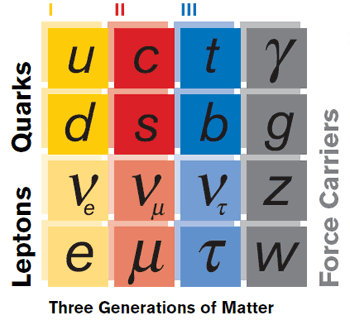
\includegraphics[width=360pt]{Figures/theory-standard-model-symmetry-mag.png}
    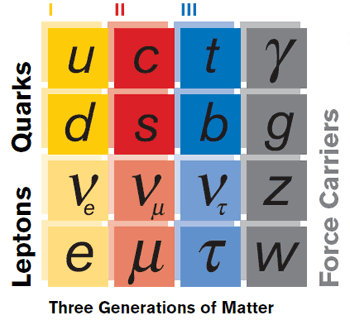
\includegraphics{Figures/theory-standard-model-symmetry-mag.png}
  \end{center}
  \caption[Particles of the standard model]
	  {Particles of the standard model that are known to exist. 
	    The Higgs boson is also predicted as part of the 
	    Standard Model, 
	    but has not yet been discovered. 

	    }
  \label{fig:StandardModel}
 \end{figure}

%antiparticles
In general, each particle has an antiparticle partner 
of the opposite charge and quantum numbers; % opposite quantum numbers in general, explain quantum numbers? because have to account for photon, gluon, Z, neutrinos
quantum numbers are used to describe the properties of the particles 
and corresponding interactions.  
For instance, all leptons have a non-zero ``lepton number;'' 
if the initial state of a set of particles 
has a total lepton number of 1, 
then any interaction between those particles will 
result in a final state with the same lepton number.  
Lepton number is always conserved in this way, 
as are charge and other quantum numbers.  
The antiparticle of the electron ($e^-$) 
has the opposite charge and lepton number 
and is called the positron ($e^+$).  
Neutrinos, being chargeless, 
have antineutrinos with opposite lepton number.  % EXPLAIN!!!!!
Quarks and gluons have another quantum ``number'' known as color.   % EXPLAIN HOW CANNOT HAVE BARE QUARKS
The three colors are red, green, and blue, with the corresponding 
``anti-colors'' being anti-red, anti-green, and anti-blue.  
%This ``color'' does not refer to our everyday experience of red, green, and blue, 
%%but there is a certain analogy to light in the ``quantum color'' behavior.  
%but the name is not accidental -- there is an analogy to colored light.  
Color is unique in that all observed states of quarks and gluons 
are ``colorless.''
In two-quark states, a color and its anti-color ``combine'' to make a colorless state.  
Three-quark states are also colorless, but through a different combination: 
the three quarks are colored red, green, and blue 
(or the corresponding anticolors), which ``combine'' (like colored light) to form 
a state with no color.
  
Not shown in Figure~\ref{fig:StandardModel} is the Higgs boson, 
which is predicted by the Standard Model 
to give mass to the other particles.  
The Higgs has not yet been discovered; 
finding it (if it exists) is one of the 
goals of the LHC.  

The Standard Model does not include the final 
fundamental force, gravity.  
Gravity is the weakest of the forces and does not 
measurably affect interactions between fundamental particles.  
The reason that it is the only one observable on a 
cosmological scale is because its ``charge,'' mass, 
is cumulative; there is no anti-mass to counter it 
the way a negatively-charge electron and a positively-charged 
proton combine to make an electrically neutral hydrogen atom.  % put this sort of stuff in beginning?
Gravity has been described on a macroscopic scale, but 
%so far gravity has not yet been (fully?) worked into the % FIXME!!!
%framework of the fundamental particles.  
so far no theory has fully united gravity with the 
other fundamental forces.  
%There are many efforts currently ongoing to unite them, % REFERENCE?
%but none of these approaches have yet been proved.  
Such a ``theory of everything'' is 
%a dream of 
one of the goals that 
theoretical physics %.  
pursues.  

% http://www.symmetrymagazine.org/cms/?pid=1000064  the symmetry magazine SM picture
% don't know how it prints in black and white
% LATEX DOESN'T DO GIFS

TABLE OF MASSES




gauge groups, little intro to group theory

A ``group'' is a set of elements with specific properties.  
In particular, any transformation of an element in the group 
results in another element in the group.  

A ``Lie'' group is one in which any transformation % NEED THIS????
can be done in very small steps, 
each of which results in an element still in the group.  
The different fundamental forces are described by different Lie groups.  

which particles feel which forces?

Each of the three forces in the Standard Model 
is described by such a Lie group.  % group. 
%In each case, the ``dimension'' of the group 
%is the dimension of the matrices
Each group is represented by a set of square matrices 
of some dimension, given by the number in parentheses.  
The matrices used for these representations are 
all unitary (hence the common ``U'' designation).  
``Unitary'' means that the matrix's inverse 
is equal to its complex conjugate transpose.  
In other words, if you flip the matrix's elements 
about its diagonal and replace each imaginary unit $i$ 
with $-i$, then multiply it by the original matrix, 
the result is the identity matrix.   % EXPLAIN IDENTITY MATRIX??

%EM: U(1)
The electromagnetic force is described by the $U(1)$ group.  
Essentially, this describes rotation about an axis.  % talk about more than matrices?
The single parameter (an angle) requires only one matrix, 
corresponding to a single % force particle(s)
force carrier, the photon.  
The electromagnetic force causes interactions between 
photons and any particles that have electric charge.  
This includes quarks, leptons, and the charged weak bosons.  
%Because the photon is massless, the electromagnetic force % EXPLAIN MORE???
%can act over long distances, observable on the human scale.  

%Weak: SU(2)
The weak force is represented by the $SU(2)$ group.  
The ``S'' addition in the name stands for ``special'' 
and means that each matrix's trace 
(the sum of elements along the matrix's diagonal) is zero.  
$SU(2)$ represents rotations in three dimensions 
using three matrices, 
and therefore has three parameters corresponding 
to the single angle of $U(1)$.  
These give rise to the three carriers of the weak force, 
the two oppositely-charged W's and the Z.  %%% FIGURE OUT HOW TO DO W+- in latex? sort of like writing it out longhand, but should show at least W+ and W- notation 
%All three carriers have significant mass, which means 
%the distance over which they have an effect is very small.  
The weak force acts on any particles that have the ``weak 
version'' of electrical charge, 
namely all fermions.  
In particular, the weak force is the only way 
neutrinos interact.  
%However, interactions with W's only happen in ways  % TALK ABOUT CONSERVATION OF CHARGE IN GENERAL
%that conserve charge.  

%QCD: SU(3)
Finally, the strong force is represented by $SU(3)$, 
which does not have an easy analogy to rotations 
like the previous two groups.  
It uses eight matrices, which correspond to the 
eight different gluon states that mediate the force.  
% talk about dim-3 = 3 colors?
The three dimensions of the group relate to the 
three ``color charges,'' red, green, and blue.  
Strong force interactions happen between all particles 
that carry this color charge, 
namely quarks, but also gluons themselves.  
% talk about color confinement and asymptotic freedom?  YES, but how to explain in terms of mass???
This so-called self-interaction on the part of the gluons 
causes the strong force to increase with distance.  
At short distances, the quarks making up another particle 
essentially act free; 
only when they get further apart do they feel the force 
keeping them in their bound state.  
This situation is related to the fact that quarks are 
never observed alone, only within these bound states.  
An interaction that is energetic enough to cause 
quarks to separate is also energetic enough to 
create more quarks with which the original quarks 
form new bound states.  
%When a quark gains a significant energy 
%(through an interaction with another particle), 

%This is known as color confinement
%The implication is that in spite of the fact that 
%gluons are massless, 
%the strong force is not observable over large distances.  

However, the individual groups by themselves 
do not necessarily represent the reality of particles.  
It is known experimentally that the bosons carrying 
the weak force have mass.  
%The $SU(2)$ formulation of the weak force
In order for the theory to correctly predict the 
fact those particles should be massive, 
the electromagnetic and weak interactions had to be combined 
into a single framework, 
%Steven Weinberg and Abdus Salam 
%The electromagnetic and weak forces were combined into one framework, 
$SU(2) \times U(1)$, using a specific method.  
The integrated $SU(2) \times U(1)$ group 
allows for the collective four force-carrying bosons 
(photon, positively- and negatively-charged W's, and Z) 
to be described as compositions of the same underlying states.  
The fact that the three weak bosons are massive, though, 
comes from applying ``spontaneous symmetry breaking.''  
This method uses the fact that the groups mentioned 
above have underlying symmetries: 
that is, they contain parameters that do not affect the 
physical description in any way.  
They are symmetric with respect to variations in these parameters.  
However, the values of these parameters can be chosen 
in a strategic way and the result manipulated % TALK ABOUT FIELD THEORY AT ALL?? this is all lagrangians and mass terms
to give masses to the weak bosons.  
(A consequence of this ``strategic choice'' is the appearance 
of another massive particle in the theory: 
the Higgs boson.  
The Higgs boson is therefore predicted by the theoretical 
mechanism used to account for massive weak bosons.  
Time -- and collision data -- will tell if the theory 
in this form is correct.)  


%Transformations within these groups can be represented as matrices.  % IS THIS ACTUALLY THE SAME AS THE GROUP MATRICES??
These matrices act on the set of initial states 
and result in the set of final states.  
Each element in the matrix, mapping a single initial state 
to a single other final state, 
gives the amplitude with which the % ONLY IN SCATTERING???  make sure this is right context 
transformation happens.  
Essentially, squaring the matrix element gives the 
relative probability of that particular transformation.  
Matrices are often used to represent transitions 
from one quantum mechanical state to another.  

This is used in particle physics as such: 
a transformation from an initial state, 
in our case two quarks from colliding protons, 
to a final state, 
an electron and a positron, 
is represented by a Feynman diagram, 
shown in Figure~\ref{fig:ZeeFeynmanDiagram}.  
The interaction can be thought to progress to the right.  
Each straight line represents a fermion, 
either the quark or the electron.  
The wavy line represents a boson, the Z.  
(Gluons are represented by curly lines.)  
The intersections between particle lines, or vertices, 
show interactions between the given particles.  
%The type of interaction can be determined by the particles   % NEED THIS?  
%taking part: 
%an interaction between a Z and a quark or lepton 
%indicates the weak force is involved.  
The matrix element corresponding to this transformation 
can be written down 
by attributing factors to the various elements 
of the Feynman diagram, 
the particle lines and the vertices.  

somewhere get into spinors...

put equation for differential cross section element 
in terms of amplitude/matrix element 



put all qcd stuff in here?  don't need all the detail of zeus stuff

\section{Electroweak Physics}
\label{theory:EWK}

lagrangian etc? i.e. more specifics on ewk physics

feynman diagrams, how they can actually be used -> 
matrix elements -> cross section element.  

\begin{figure}[htb]
\begin{center}
  \begin{tikzpicture}[
      thick,
      % Set the overall layout of the tree
%      level/.style={level distance=1.4cm, line width=0.8mm},
      level/.style={level distance=1.4cm, line width=0.5mm},
      level 2/.style={sibling distance=1.4cm},
      level 3/.style={sibling distance=1.4cm}
    ]
    \coordinate
%    child[grow=south east]{
%      child[grow=north east]{
%        edge from parent [gluon]
%        node[right]{$g$}
%      }
    child[grow=south east]{
      edge from parent [electron]
      child[grow=south west] {
        edge from parent [electron]
%        node[above] {$\bar{q}$} % ADDED
        node[below] {$\bar{q}$} % ADDED
%          child[grow=south west]{
%            edge from parent [electron]
%            node[above] {$\bar{q}$}
%          }
%          child[grow=south east]{
%            edge from parent [gluon]
%            node[right] {$g$}
%          }
      }
      child[grow=east, level distance=2.4cm] {
        child[]{ % added the [], did nothing, don't know how to make angle of line the same as LHS
          edge from parent [electron]
          node[below] {$e^{-}$}
        }
        child[]{ % added the [], did nothing, don't know how to make angle of line the same as LHS
          edge from parent [electron]
          node[above] {$e^{+}$}
        }
%        edge from parent [boson]
        edge from parent [zboson]
%        node[below] {$Z/\gamma*$}
        node[below] {$Z$}
      }
%    }
      edge from parent [electron] node [above=3pt] {$q$}
    };
  \end{tikzpicture}
\end{center}
%  \caption[Feynman diagram of \qqZgee]
  \caption[Feynman diagram of \qqZee]
%	  {Feynman diagram of \qqZgee.  
	  {Feynman diagram of \qqZee.  
	    }
  \label{fig:ZeeFeynmanDiagram}
\end{figure}

where to put cross section formula stuff 
-- make new section?
(and which stuff to use?)

order of diagram = number of vertices!  

\subsection{Z Production}
\label{theory:Zprod}

someplace need to go into 4-momenta...

s, inv mass, pdfs attach to tree-level matrix element, 
Z/gamma* interference

s = Z mass -- well, dunno, also includes momentum

The quantity $s$ is the square of the center-of-momentum 
energy of the colliding proton system.  
(Therefore $\sqrt{s}$ is the center-of-momentum 
energy itself.)  
It is obtained by adding together the four-momenta 
of the colliding protons, designated $1$ and $2$: %.  
\[
s = (p_1 + p_2)^2
\]
However, since only a single quark participates 
in the interaction, not the full proton, 
the energy of the interaction must be reduced.  
The fraction of the proton's momentum that is carried 
by the quark is defined $x$, so that the 
quark's momentum is then $xp$.  
We can then define a center-of-momentum energy, 
$\hat{s}$ (or $Q^2$), 
for the quark-quark system, 
the interacting part of the proton system: 
\[
\hat{s} = (x_1 p_1 + x_2 p_2)^2
\]
This can be approximated in terms of the original 
(proton) $s$ as 
\[
\hat{s} \simeq x_1 x_2 s
\]





!!!! THIS IS ALL FOR PHOTONS DRELL YAN !!!!!
is that okay?????????
Z's have different feynman rule factors!!


more specific derivation stuff?  
I guess, if I'm starting from the 
feynman diagram stuff

% the VERY beginning of the cross section formula
% where |M|2 is ``probability'', F is flux = particles per area per time, 
% and dQ is dLIPS
\[
d \sigma = \frac{ \left| \mathcal{M} \right| ^2 }{F} d Q
\]

% (in CM) the full differential cross section is 
\[
\frac{d \sigma}{d \Omega} \big| _{CM} 
= \frac{1}{64 pi^2 s} \frac{p_f}{p_i} \left| \mathcal{M} \right| ^2
\]
% where d\Omega is solid angle element
% pf and pi are the initial and final momenta of each element,
% since in CM pi1 = pi2, pf1 = pf2
% differential is eventually integrated

%% % now for curly M squared
%% % Feynman diagram sez 
%% \[
%% \mathcal{M} = -
%% \]

curly M can be written down from Feynman rules, 
according to tensor structure



the giant thing from the PDG RPP CH 40:

partial width given by 
\[
\Gamma(Z \rightarrow f \bar{f} )
= N_c \frac{ \sqrt{2} G_F m_Z^3 }{6 \pi}
\times \left[(T_3 - Q_f \sin^2 \theta_W )^2 
+ (Q_f \sin \theta_W )^2 \right]
\]
while the giant thing is given by 
(full differential cross section for 
$ f_i \bar{f_j} \rightarrow (W,Z) \rightarrow f_{i'} \bar{f_{j'}} $)
\[
\frac{d \sigma}{d \Omega} = \frac{N_c^f}{N_c^i} 
\times \frac{1}{256 \pi s} 
\times \frac{s^2}{(s - m_Z^2)^2 + s \Gamma^2}
\times \left[(L^2 + R^2) (L'^2 + R'^2) (1 + \cos^2 \theta)
+ (L^2 - R^2) (L'^2 - R'^2) 2 \cos \theta \right]
\]
For Z, couplings are 
\[
%L = \sqrt{ \frac{8 G_F m_Z^2}{\sqrt{2} } }(T_3 - \sin^2 \theta_W Q)
L = g (T_3 - \sin^2 \theta_W Q)
\]

\[
%R = - \sqrt{ \frac{8 G_F m_Z^2}{\sqrt{2} } } \sin^2 \theta_W Q
R = - g \sin^2 \theta_W Q
\]
``$T_3$ is weak isospin of initial left-handed fermion and 
Q is initial fermion's electric charge. [FRACTIONAL] 
The expressions for L' and R' are analogous.  
The color factors $ N_c^{i,f} $ are 3 for initial or final quarks 
and 1 for initial or final leptons.''  

$T_3$ is the third component of the ``weak hypercharge,'' 
which relates how to the fermions are arranged 
within the standard model generations 
(refer to Figure~\ref{fig:StandardModel}).  
Each generation consists of two pairs, 
one pair of quarks and one pair of leptons.  
The placement of each particle within its pair 
reflects how it interacts with the weak force.  
This quantity is the ``weak version'' of electric charge, 
known as ``hypercharge.''  
For the top particle in each pair, the hypercharge 
is $+\frac{1}{2}$; 
for the bottom particle, it is $-\frac{1}{2}$.  
(Note: this only applies to particles whose spin 
is ``left-handed.''  
Particles with ``right-handed'' spin have zero hypercharge; 
right-handed neutrinos do not interact in the Standard Model.  
This is equivalent with the assertion that neutrinos 
must be moving at the speed of light and therefore 
do not have mass. 
If neutrinos had mass, 
they would be moving slower than the speed of light 
and there could be a reference frame -- 
where the observer moves faster than the neutrino -- 
in which the neutrino would actually be left-handed.  
Because recent observations have indicated neutrinos % REFERENCE
do in fact have mass, 
this aspect of the Standard Model is inaccurate.)  
%H+M have SUCH a nice little summary in the inside back cover.  

can put in terms of little g:
\[
g = \sqrt{ \frac{8 G_F m_Z^2}{\sqrt{2}} }
\]
Initial particles are quarks: 
\[
N_c^i = 3
\]
Final particles are leptons: 
\[
N_c^f = 1
\]
BUT, initial particles are all flavors of quarks, 
so can't just plug in flavor-dependent quantities 
like $T_3$ and $Q$.  



%% % WHICH simplifies to give us AVGD OVER SPINS or whatever
%% \[
%% \bar{ \left| \mathcal{M} \right| ^2 } 
%% = 2 e^4 \left[ \frac{1}{2} \left( 1 + \cos^2 \theta \right) \right]
%% \]

%% % THEN
%% \[
%% \frac{d \sigma}{d \Omega} \big| _{CM}
%% %= \frac{\alpha^2}{4s} \left( 1 + \cos^2 \theta \right) 
%% = \frac{\alpha^2}{4 Q^2} \left( 1 + \cos^2 \theta \right) 
%% \]


% quark-level subprocess is 3 e_q^2 times that for muons
% DON'T NEED TO SHOW THIS, backwards anyhow
%\[
%\sigma(e^- e^+ \rightarrow q \bar{q} ) 
%= 3 e_q^2 \sigma(e^- e^+ \rightarrow \mu^- \mu^+ )
%\]

%% % WHERE
%% %\[
%% %\sigma(e^- e^+ \rightarrow \mu^- \mu^+ ) 
%% %= \frac{4 \pi \alpha^2}{3 s}
%% %\]
%% % don't need to show that one either, 
%% %just result: 
%% \[
%% \sigma ( q \bar{q} \rightarrow e^- e^+ )
%% %= 3 e_q^2 \frac{4 \pi \alpha^2}{3 s}
%% = 3 e_q^2 \frac{4 \pi \alpha^2}{3 Q^2}
%% \]
%% % D'OH, look at next line!

%% % cross section of quark-level subprocess
%% \[
%% \hat{\sigma} (q \bar{q} \rightarrow l^- l^+) 
%% = \frac{4 \pi \alpha^2}{3 Q^2} e_q^2
%% \]

% but need to account for the proton and pdfs

\[
\frac{d \sigma}{d Q^2}(pp \rightarrow l \bar{l} X)
= \left( \frac{1}{3} \right) \left( \frac{1}{3} \right) 3 
\sum_q \int dx_1 \int dx_2 f_q (x_1) f_{\bar{q}} (x_2)
\frac{d \hat{\sigma} }{d Q^2}
\]

%% % ... which gives
%% % THE BIG FAT GIANT CROSS SECTION EQUATION 
%% % in terms of the parton distribution functions f_i(x)
%% \[
%% \frac{d \sigma}{d Q^2}(pp \rightarrow l \bar{l} X)
%% = \frac{4 \pi \alpha^2}{9 Q^4} 
%% \sum_q e_q^2 \int dx_1 \int dx_2 f_q (x_1) f_{\bar{q}} (x_2) 
%% \delta \left( 1 - x_1 x_2 \frac{s}{Q^2} \right)
%% \]

% THIS IS ONLY LOWEST ORDER, with no ISR/FSR gluon emission stuff

%do I have to go all the way through the cross section stuff???  yeah, I think so...


%The definition of a 
A particle system's ``invariant mass'' is 
a combination of its energies and momenta that 
remain unchanged regardless of reference frame.  
A particle (or everyday object) can appear to 
have a different energy depending on the reference 
frame from which it is viewed.  
If you are sitting on an airplace at cruising altitude, 
the plane is not moving with respect to your body.  
However, if you are on the ground, the plane is 
moving very fast -- 
it has a different kinetic energy in that frame.  
The physics of the situation cannot depend on 
the reference frame of the observer, 
even at the relativistic speeds of interacting particles.  
The invariant mass is such a quantity that 
remains the same.  
In addition, since the energy and momentum 
of a system are conserved, 
the invariant mass is also conserved 
throughout the entire interaction, 
in particular the decay.  
The general definition is given as 
\[
M_{inv}^2 = \left( \sum E \right)^2 - \left\| \sum \mathbf{p} \right\|^2
\]
For a single particle, the expression simplifies 
to the particle's mass.  
This analysis makes use of the fact that the 
invariant mass of the decay particles 
(the two electrons) 
is the same as the (invariant) mass of the 
particle which decayed, the Z.  
The above formula, simplified to two particles, 
\[
M_{inv} = \sqrt{ \left(E_1 + E_2\right)^2 - \left\|\mathbf{p}_1 + \mathbf{p}_2\right\|^2 }
\]
reconstructs the mass of the Z boson 
based on the energies and momenta 
of the decay products.  

Another diagram contributes to the process being studied. 
In this case, a photon replaces the Z boson 
as the link between the quarks and the electrons.  
Because these diagrams have the exact same 
initial and final states, 
they ``interfere'' with each other.  
Experimentally, it is impossible to tell which one happened; 
both must be included in the calculations.  % is this exactly why???

It is necessary to note that the photon that takes 
part in this interaction is a ``virtual'' photon -- 
%it cannot be observed by itself.  
it cannot be directly observed.  
The reason for this is that there is always a 
center-of-momentum reference 
frame for the two particles colliding to form the photon.  
In other words, there is always some way that you, 
the observer, can be moving, 
such that it looks like the two particles 
have the same speed but opposite directions.  
In this reference frame, the photon would be formed at rest, 
which violates the principle that the speed of light 
is the same in all reference frames -- 
the speed of light can never be zero.  
Equivalently, such a photon would have mass, 
while real photons are massless.  
The mass of this virtual photon is indeed the same 
as the invariant mass of the system.  
%Such virtual particles can exist due to inherent   %% is that actually why these photons in particular can be virtual?  
%fluctuations in energy, by the uncertainty 
%principle of quantum mechanics.  
Such virtual particles are allowed to exist 
by the uncertainty principle of quantum mechanics, 
which governs the ``borrowing'' of energy from the vacuum.  
The smaller the time scale over which the energy 
fluctuation happens, 
the larger the energy fluctuation allowed.  

Having a specific mass defines a thin 
surface or ``shell'' in kinematic phase space; 
only certain combinations of energy and momentum 
are allowed, 
because of the relations between mass, energy, and momentum.  
Particles that are virtual, 
i.e. have a mass much different than their 
defined ``real'' mass, 
are called ``off-shell'' -- 
they are ``off the mass shell.''  

The Z boson, while it has a defined mass, 
%DECAY WIDTH ETC ETC ETC 
can be ``off-shell'' in the same way as the photon.  
That is, in general the 
%reconstructed 
mass 
does not take on a single precise value; 
instead, over many events it manifests as a distribution 
peaked around the ``real'' value.  
This is typical of particles that are measured only 
by their decays; 
these particles tend to be at least slightly virtual 
%because they are not being observed directly.  
because of their short lifetimes.  
%in fact, 
%In addition, the width of the peak is inversely related to the   % how relevant is this actually?  
%lifetime of the particle.  

PIC OF DY SPECTRUM??

In this case, only the area around the Z peak is being 
studied, not the full spectrum.  
The main contribution in this area is the Z itself 
as opposed to virtual photons.  


\subsubsection{Results from Previous Experiments}
\label{theory:prev}

\subsection{Z Decay}
\label{theory:Zdec}
need this section??


somewhere have intro to QFT and all that?  

also, explanatory items from overview:

   * [here or] in theory chapter define ``tree-level''.  
ALSO IN THEORY: explain how Feynman diagrams are so useful! 
writing down the matrix element and all that
AND PDFs, basically whole process of stuff simulated 
really happens and should be explained.  
AND DEF OF PARTONS
yeah, basically explain all the stuff in the MC chapter
INCLUDING ISR and FSR
ALSO define ``jets'' and talk about how they come from 
quarks and gluons (define partons) and relate to ``hadronization'' -- 
not entirely relevant for this analysis, 
but possible in general
AND define ``color''
AND asymptotic freedom, how it takes more and more energy to get them further apart

   * intial- and final-state radiation

   * [HERE OR IN THEORY INTRO] need to do on-shell/off-shell decays 
to explain why Z mass has a spectrum and not a single value

   * invariant mass (here?)

   * cross section formula and matrix elements and what said matrices do

   * PDFs, what they are, how they relate to Z physics

AND, of course read the others' theses to see what they had in here, too.  



